\subsection{Tracks}\label{HiC:tracks}% __03a-tracks
%~~~~~~~~~~~~~~~~~~~%
\subsubsection{Input} % inputs
Data from the pipeline \texttt{filter} step is used as input (Section~\ref{HiC:filter}).
%~~~~~~~~~~~~~~~~~~~%
\subsubsection{Analysis} % analysis
Default parameters:
\begin{lstlisting}
params.standard.tcsh$
#!/bin/tcsh

source ./inputs/params/params.tcsh

set bin_size = 40000                # this is a commonly used bin size
\end{lstlisting}
%~~~~~~~~~~~~~~~~~~~%
\subsubsection{Output} % outputs
Default output: % results/tracks.by_group.standard/filter.by_sample.standard/align.by_sample.bowtie2/CD34-HindIII/
\begin{lstlisting}
-rw-r--r--  1 at570 4.1K Jan 13 15:55 job.err
-rw-r--r--  1 at570   47 Jan 13 15:10 job.id
-rw-r--r--  1 at570    0 Jan 13 15:11 job.out
-rw-r--r--  1 at570  242 Jan 13 15:10 job.sh
-rw-r--r--  1 at570 2.6K Jan 13 15:55 job.vars.tsv
-rw-r--r--  1 at570 1.1G Jan 13 15:54 track.washu.tsv.gz
-rw-r--r--  1 at570 789K Jan 13 15:55 track.washu.tsv.gz.tbi
\end{lstlisting}
\begin{figure}[!htb]
    \centering
    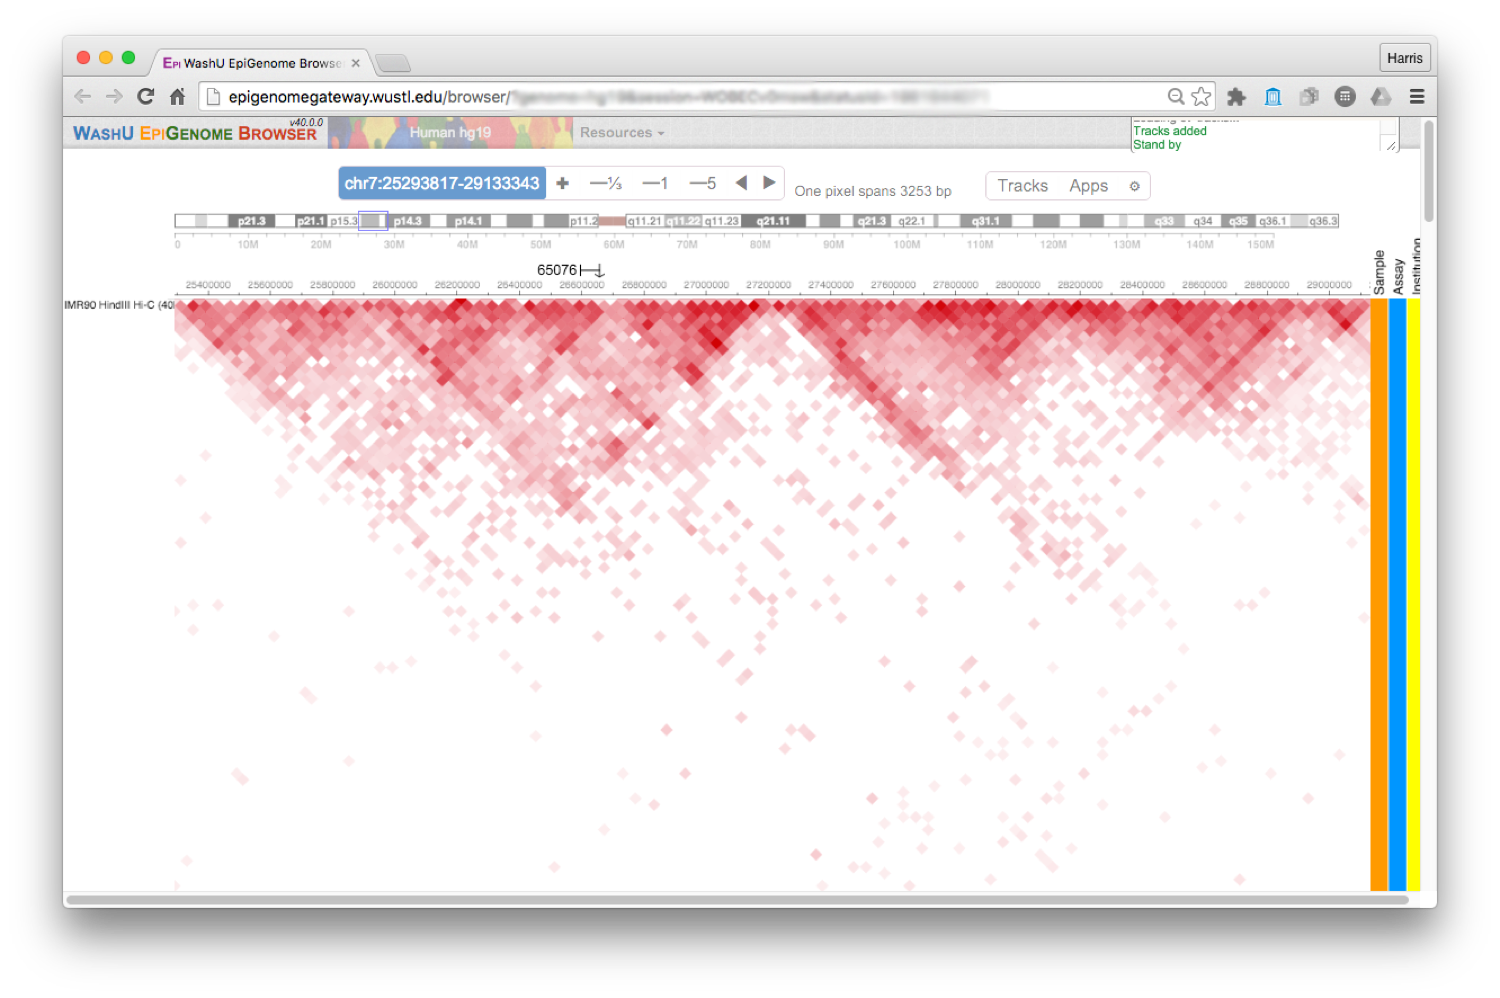
\includegraphics[width=\textwidth,height=\textheight,keepaspectratio]{figure/WashU_session}
    \caption{WashU tracks loaded in browser.} %from powerpoint
    \label{fig:hicplotter_chr8}
\end{figure}
% \newpage
\clearpage